\documentclass{beamer}
\usepackage[spanish]{babel}
\usepackage[utf8]{inputenc}
\usepackage{graphicx}

\title[Series de Taylor en \textsc{Beamer}]{Series de Taylor en la función arcsin(x)}
\author[A. Gómez, S. Luis y S. Verona]{Ana Gómez Pérez, Sara Luis Farrais y Shaila Verona Rodríguez}
\date[11/05/14]{11 de mayo de 2014}
\usetheme{Madrid}

\definecolor{ColorGris}{RGB}{56,61,66}
\setbeamercolor*{palette primary}{use=stucture, fg=white, bg=ColorGris}

\begin{document}

\begin{frame}

\includegraphics[width=0.15\textwidth]{ull.jpeg}
\hspace*{7.5cm}

\includegraphics[width=0.15\textwidth]{indice.jpeg}
\hspace*{7.5cm}
\titlepage
\end{frame}

\begin{frame}
\frametitle{Índice}
\tableofcontents[pausesections]

\end{frame}

\section{El método de Taylor}

\begin{frame}
\frametitle{El método de Taylor}
El método de Taylor es uno de los algoritmos más antiguos utilizados para aproximar la solución de un problema de valor inicial en una ecuación diferencial ordinaria.

\begin{block}{Fórmula del polinomio de taylor}
$$p(x)=f(a)+\frac{f'(a)}{1!}*(x-a)+\frac{f''(a)}{2!}*(x-a)^2+\frac{f'''(a)}{3!}*(x-a)^3+...+\frac{f^n(a)}{n!}$$ 
\end{block}

\end{frame}

\begin{frame}
\frametitle{El método de Taylor}
El metodo de Taylor es una representación de una función como una infinita suma de términos.
Estos términos se calculan a partir de las derivadas de la función para un determinado valor de la variable (respecto de la cual se deriva), lo que involucra un punto específico sobre la función.
\end {frame}



\section{Ejemplo con Taylor}

\begin{frame}
\frametitle{Ejemplo con Taylor.}

\begin{block}{}
Al aproximar con Taylor vamos a obtener otras ecuaciones según el error.
\end{block}

\begin{figure}[b]
\begin{center}
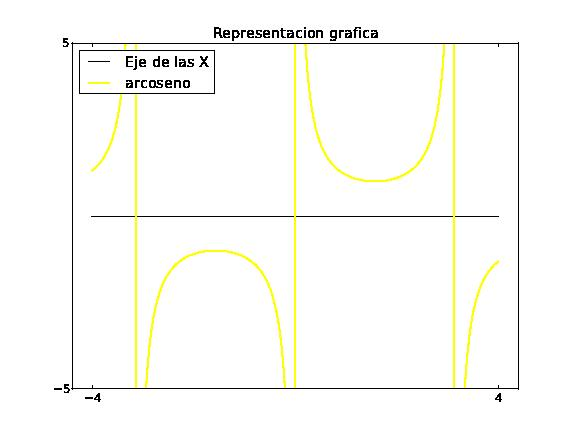
\includegraphics[scale=0.5]{grafica.jpeg}
\end{center}
\end{figure}

\end{frame}

\section{Código en Python}


\begin{frame}
\frametitle{Código en \textsf{Python}}
A continuación se muestra el código fuente creado en \textsf{Python} para la resolución del problema.

\begin{figure}[b]
\begin{center}
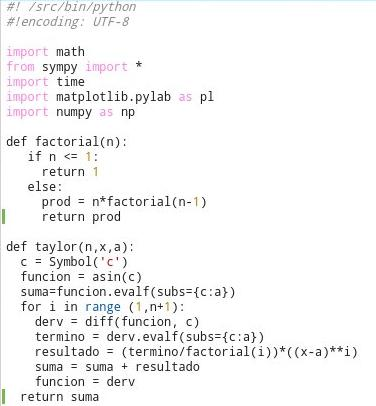
\includegraphics[scale=0.5]{py1.jpeg}
\end{center}
\end{figure}

\end{frame}



\begin{frame}
\frametitle{Código en \textsf{Python}}

\begin{figure}[b]
\begin{center}
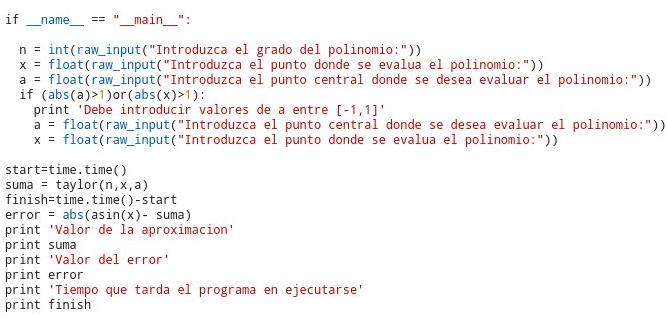
\includegraphics[scale=0.6]{py2.jpeg}
\end{center}
\end{figure}

\end{frame}

\begin{frame}
\frametitle{Código en \textsf{Python}}

\begin{figure}[b]
\begin{center}
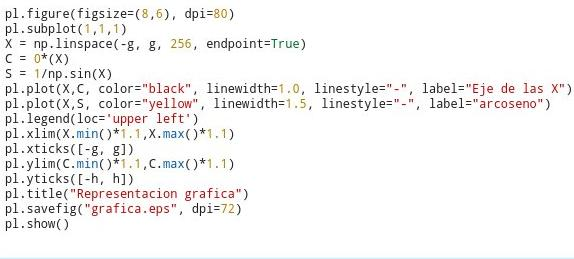
\includegraphics[scale=0.75]{py3.jpeg}
\end{center}
\end{figure}

\end{frame}

\section{La Bibliografía}

\begin{frame}
\frametitle{Bibliografía}
\begin{thebibliography}

  \beamertermplatebookbibitems
  \bibitem[Apuntes]{Análisis}
  {\small $Apuntes\_de\_la\_asignatura: Análisis\_Matemático\_II$}
  
  \beamertermplatebookbibitems
  \bibitem[Internet]{wikipedia}
  {\small $http://es.wikipedia.org/wiki/Serie\_de\_Taylor$}
  
  
  \beamertermplatebookbibitems
  \bibitem[Internet]{Biblioteca ULL}
  {\small $PuntoQ$}
  

  \beamertermplatebookbibitems
  \bibitem[Libro]{Biblioteca}
  {\small $Análisis\_Numérico\_con\_Aplicaciones. Gerald·Wheatley.$}
  
\end{thebibliography}
\end{frame}

\end{document}